\section{Ejercicio 4}

A continuación mostramos algunas corridas del algoritmo \textit{Round Robin}. Todas fueron ejecutadas con un lote de 5 tareas TaskCPU de 50 ticks de duración definidas en \textit{tareas\_ejercicio4.tsk}. En todas las corridas, tanto el costo de cambio de contexto como el costo de cambio de núcleo de procesamiento son iguales, para facilitar la lectura de los gráficos.

\subsection{Single-core}
\begin{figure}[h]
	\centering                                                       
	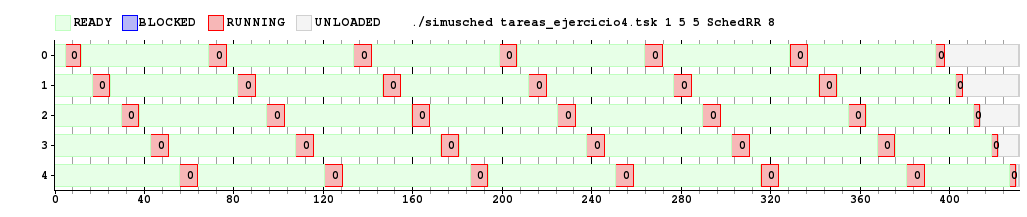
\includegraphics[width=450pt]{./figs/ejercicio4_1core.png}
\end{figure}

En esta corrida del lote se puede ver claramente el comportamiento del algoritmo \textit{Round Robin}, dado que con un quantum de 8 ticks para cada tarea, se ejecuta en el único core de prueba, alguna tarea durante ese tiempo hasta que terminan todas.

\subsection{Multi-core, igual quantum}
\begin{figure}[h]
	\centering                                                       
	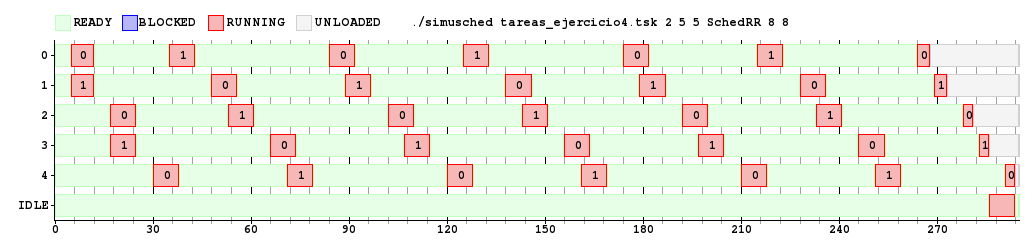
\includegraphics[width=450pt]{./figs/ejercicio4_2cores_igual_quantum.png}
\end{figure}

\begin{figure}[h]
	\centering                                                       
	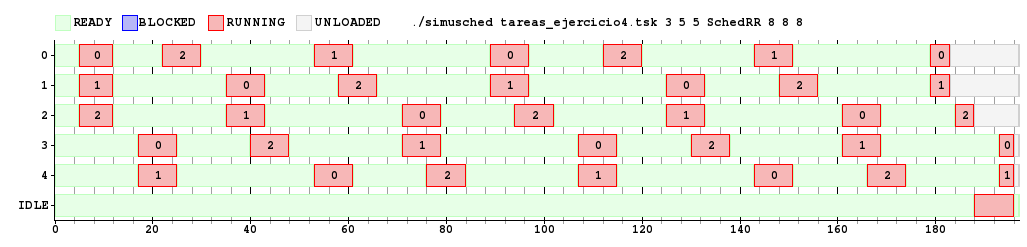
\includegraphics[width=450pt]{./figs/ejercicio4_3cores_igual_quantum.png}
\end{figure}

En estas corridas del lote se ve como se ejecutan a la vez 2 y 3 tareas durante un quantum fijo e igual para todos los núcleos. Es fácil ver como durante los primeros 2 quantums se mantiene visible el comportamiento del algoritmo. Más adelante se hace un poco más difícil de ver, pero nunca deja de apreciarse la manera secuencial característica de asignación de CPU de este algoritmo.

\clearpage

\subsection{Multi-core, distinto quantum}
\begin{figure}[h]
	\centering                                                       
	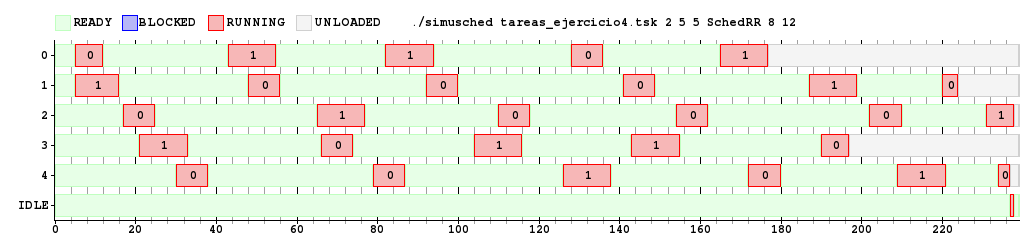
\includegraphics[width=450pt]{./figs/ejercicio4_2cores_dif_quantum.png}
\end{figure}

\begin{figure}[h]
	\centering                                                       
	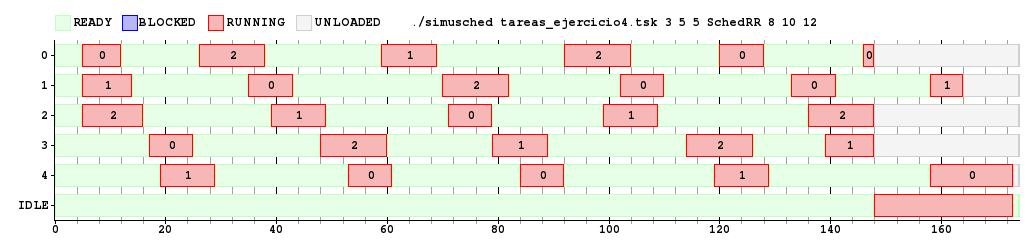
\includegraphics[width=450pt]{./figs/ejercicio4_3cores_dif_quantum.png}
\end{figure}

Estas corridas son similares a las multi-core con igual quantum. La única diferencia es el tiempo que permanece cada tarea en ejecución en alguno de los CPUs. Una misma tarea puede utilizar distinta cantidad de quantum según el core en el que se esté ejecutando. Nuevamente, se ve el comportamiento cíclico del scheduling de los procesos del algoritmo de \textit{Round Robin}.

\clearpage

\subsection{Distintas perspectivas de un mismo lote}

\begin{figure}[h]
	\centering                                                       
	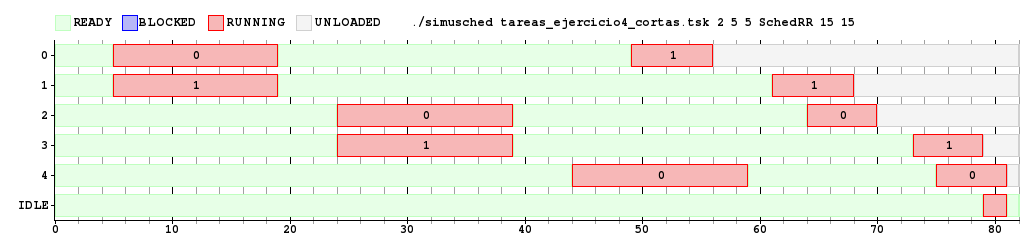
\includegraphics[width=450pt]{./figs/ejercicio4_tareas_largas.png}
\end{figure}

\begin{figure}[h]
	\centering                                                       
	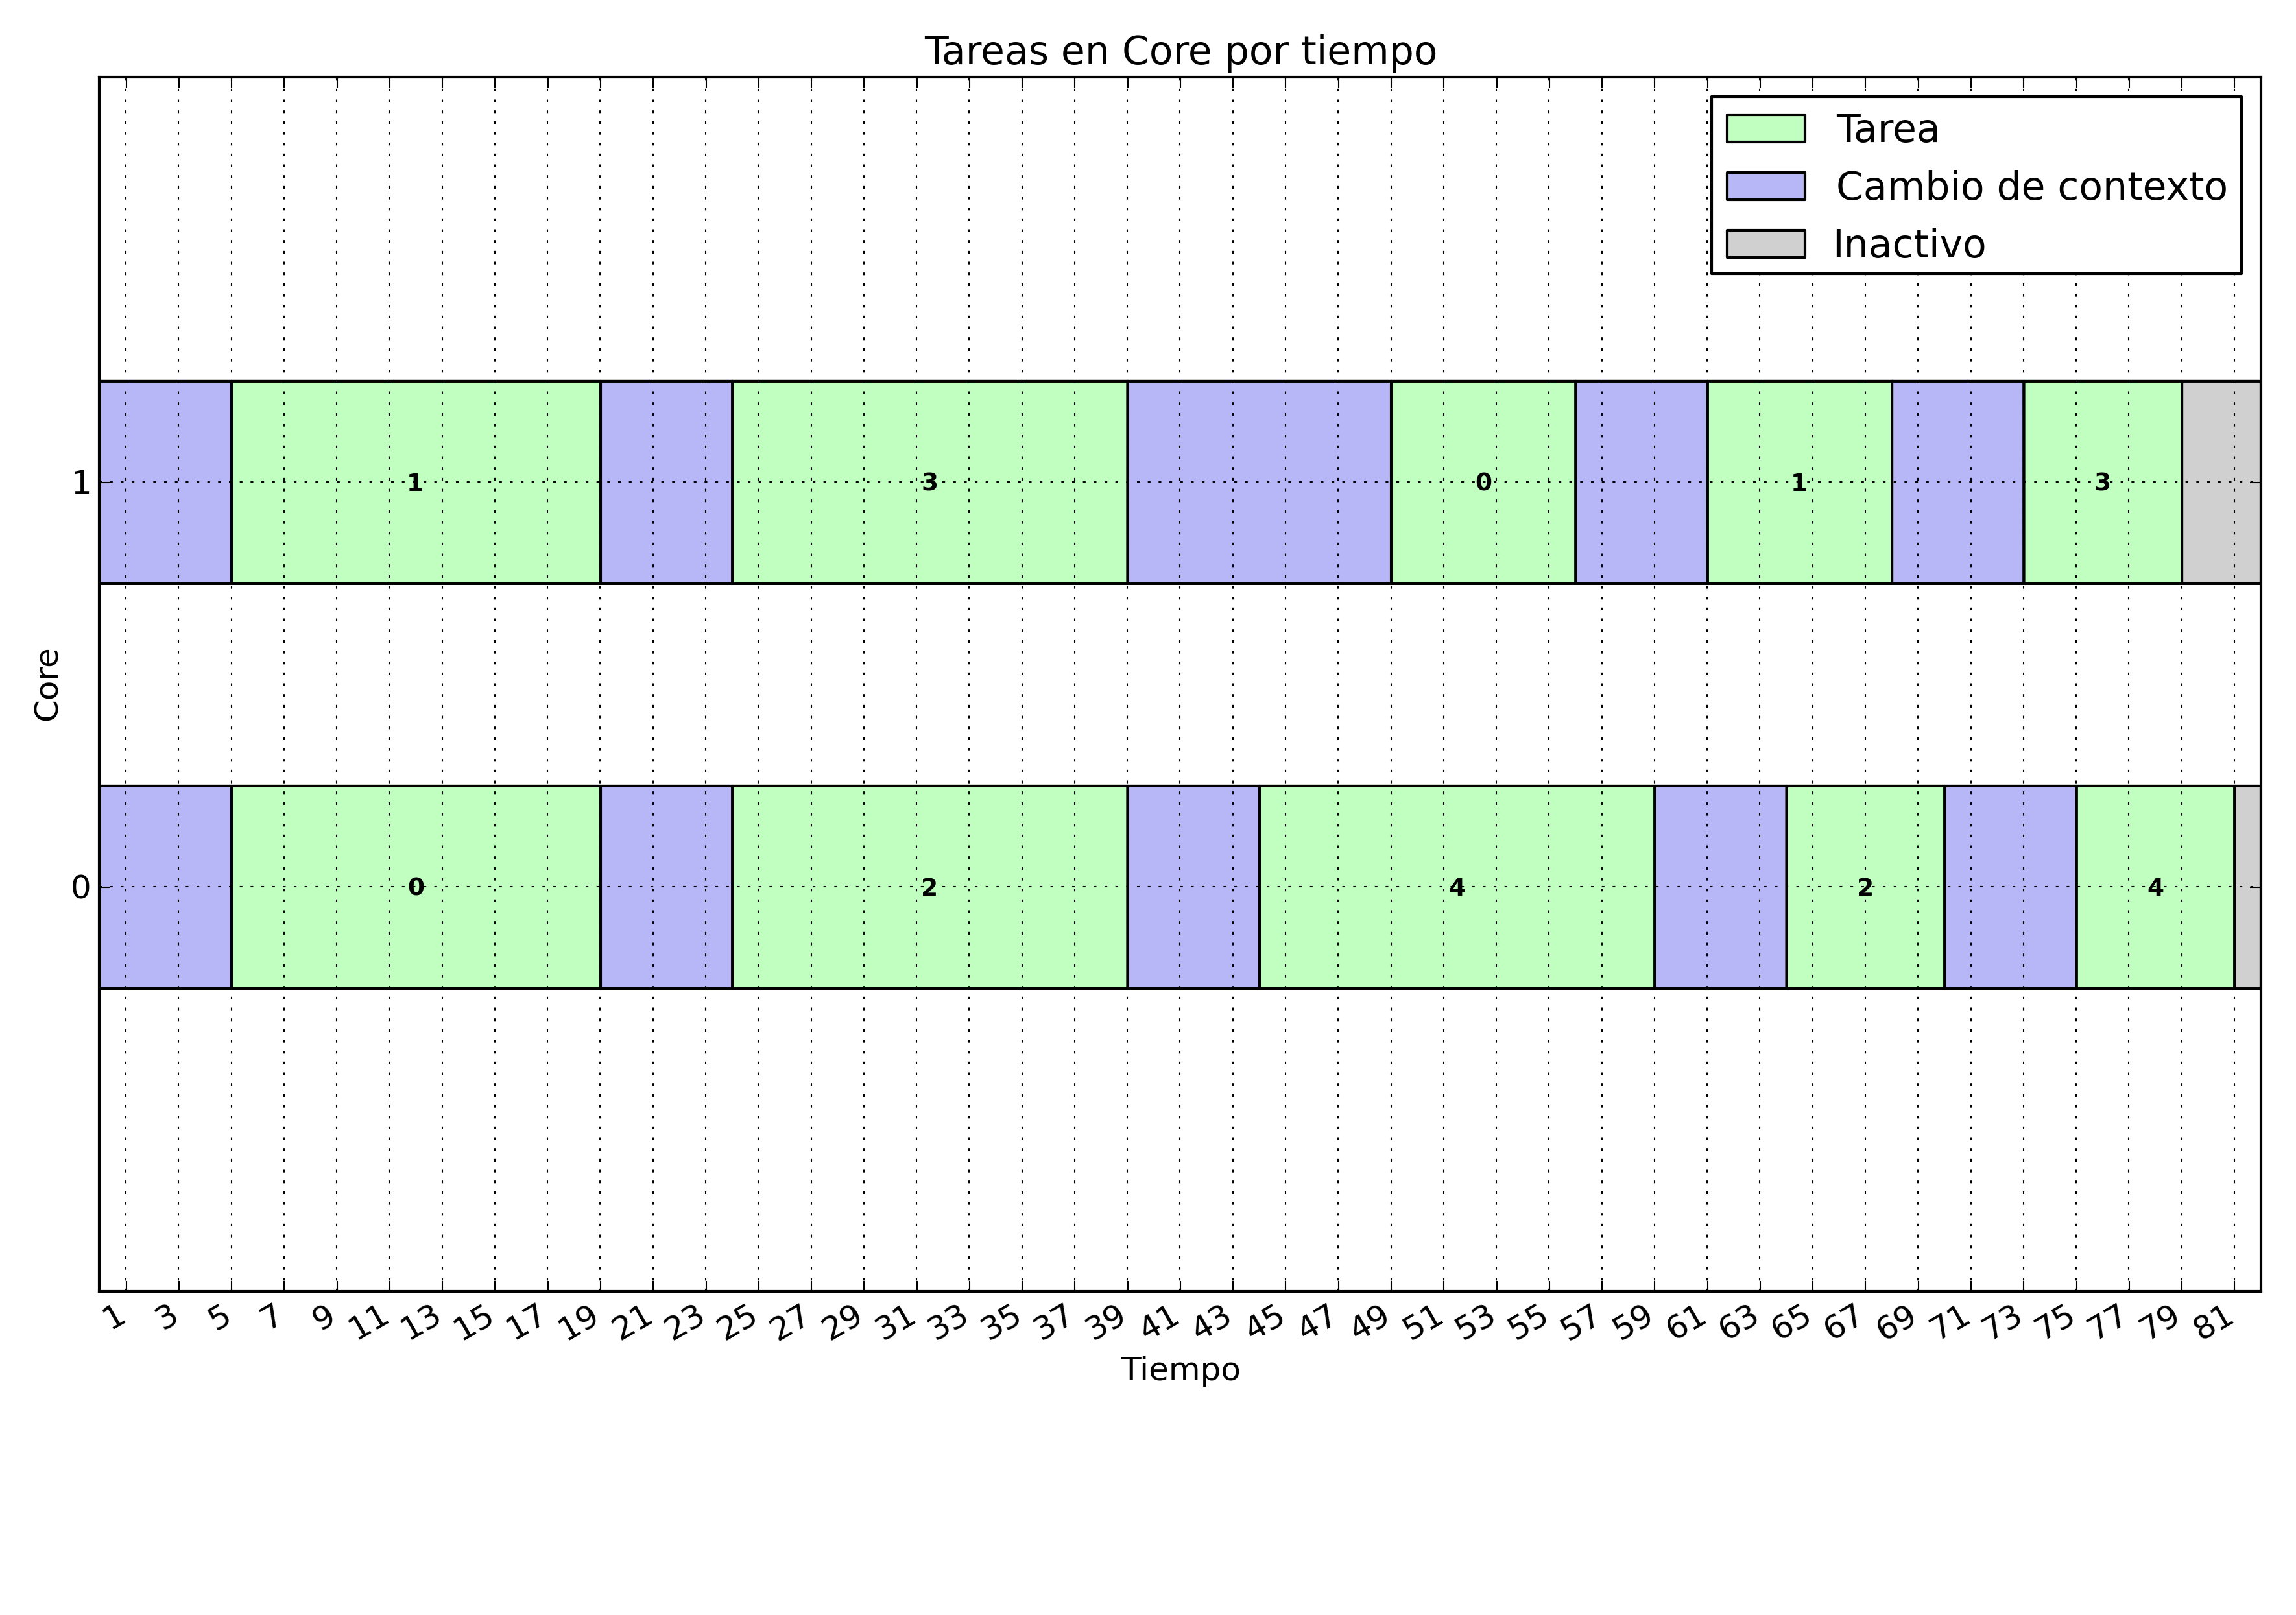
\includegraphics[width=450pt]{./figs/ejercicio4_tareas_largas_cores.png}
\end{figure}


Estos 2 gráficos son dos perspectivas diferentes de una misma corrida de un lote con 2 cores. Lo que se puede ver en el primer gráfico, es la forma en la que \textit{Round Robin} delega las tareas de manera iterativa como vimos anteriormente. En el segundo se ve la carga de cada core en un momento dado. Al ponerle el mismo quantum a ambos cores, es más fácil de ver el accionar del algoritmo.\\
\\
\indent Lo que se puede mencionar como detalle presente en estos 2 gráficos, es la forma de elegir los cores que tiene el algoritmo al finalizar su quantum por primera vez la tarea 4. Se ve claramente que, por más que al momento de ejecutarse la tarea 1 por segunda vez, el core 0 esté libre, al momento de terminar de ejecutar la tarea 0, el mismo todavía estaba siendo ocupado por la tarea 4. Por este motivo, el scheduler elige nuevamente el core 1 para trabajar, y continúa la ejecución normalmente.